\chapter{Analisi dei requisiti}
\label{cap:analisi-requisiti}

\intro{L'analisi dei requisiti è alla base della comprensione del prodotto da sviluppare, è utile per chiarire eventuali dubbi e per procedere in maniera spedita evitando perdite di tempo future}\\

\section{Casi d'uso}
%DA RISCRIVERE
Per lo studio dei casi di utilizzo del prodotto sono stati creati dei diagrammi.
I diagrammi dei casi d'uso (in inglese \emph{Use Case Diagram}) sono diagrammi di tipo \gls{uml} dedicati alla descrizione delle funzioni o servizi offerti da un sistema, così come sono percepiti e utilizzati dagli attori che interagiscono col sistema stesso.
Essendo il progetto finalizzato alla creazione di un tool per l'automazione di un processo, le interazioni da parte dell'utilizzatore devono essere ovviamente ridotte allo stretto necessario. Per questo motivo i diagrammi d'uso risultano semplici e in numero ridotto.
%ORA NON HO VOGLIA
\begin{figure}[!h] 
    \centering 
    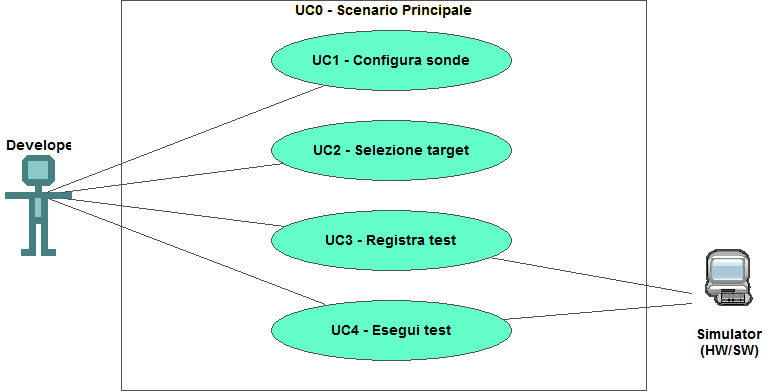
\includegraphics[width=0.9\columnwidth]{usecase/scenario-principale} 
    \caption{Use Case - UC0: Scenario principale}
\end{figure}

\begin{usecase}{0}{Scenario principale}
    \usecaseactors{Programmatore}
    \usecasepre{Il programmatore ha avviato l'ambiente di programmazione integrato}
    \usecasedesc{Avvio delle componenti base dell'applicativo}
    \usecasepost{Il sistema è pronto per eseguire il workflow}
    \label{uc:scenario-principale}
\end{usecase}

\begin{figure}[!h] 
    \centering 
    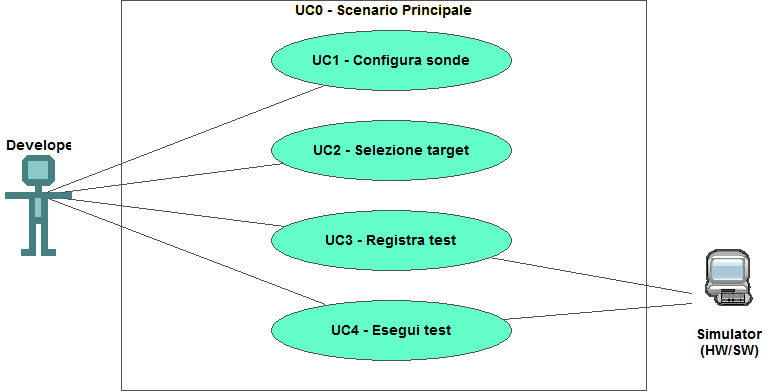
\includegraphics[width=0.9\columnwidth]{usecase/scenario-principale} 
    \caption{Use Case - UC1: Scenario principale}
\end{figure}

\begin{usecase}{1}{Acquisizione screenshot} 
    \usecaseactors{Programmatore, Web-scraper} 
    \usecasepre{Il web-scraper ha già raccolto i link alle pagine dei siti web delle aziende} 
    \usecasedesc{Il programmatore prepara il workflow per acquisire in maniera automatica gli screenshot delle pagine raccolte in precedenza} 
    \usecasepost{Gli screenshot vengono salvati nel database, pronti per la fase di analisi e classificazione} 
    \label{uc:acquisizione-screenshot} 
\end{usecase}

\begin{figure}[!h] 
    \centering 
    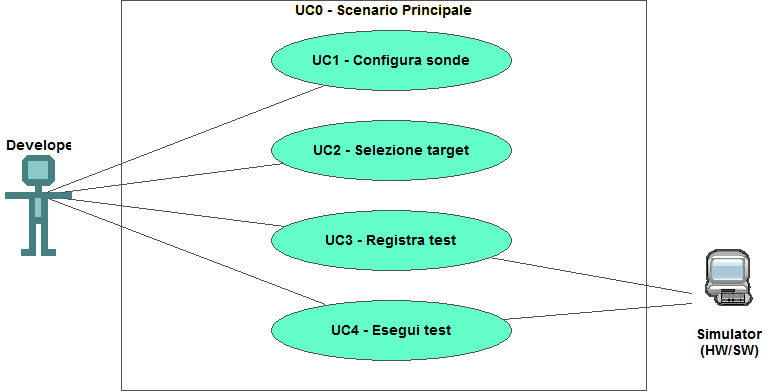
\includegraphics[width=0.9\columnwidth]{usecase/scenario-principale} 
    \caption{Use Case - UC2: Clusterizzazione degli screenshot}
\end{figure}

\begin{usecase}{2}{Clusterizzazione degli screenshot} 
    \usecaseactors{Programmatore, IA non supervisionata} 
    \usecasepre{Gli screenshot delle pagine sono stati acquisiti e salvati nel database}
    \usecasedesc{Il programmatore avvia il processo di clustering, che organizza gli screenshot in clusters in base alle feature estratte} 
    \usecasepost{Gli screenshot vengono clusterizzati e inseriti in apposite cartelle} 
    \label{uc:clusterizzazione-screenshot} 
\end{usecase}

\begin{figure}[!h] 
    \centering 
    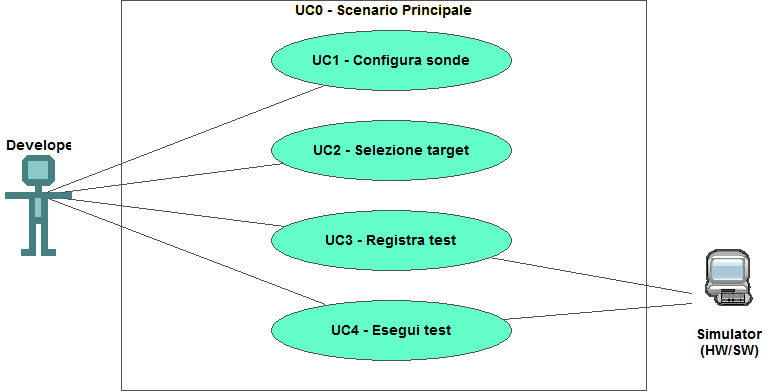
\includegraphics[width=0.9\columnwidth]{usecase/scenario-principale} 
    \caption{Use Case - UC3: IA classificativa}
\end{figure}

\begin{usecase}{3}{Valutazione qualitativa e classificazione} 
    \usecaseactors{Programmatore, IA classificativa} 
    \usecasepre{Gli screenshot sono stati inseriti in cartelle} 
    \usecasedesc{Lo sviluppatore addestra l'IA classificativa sfruttando i cluster precedentemente creati, e creando un dataset} 
    \usecasepost{Ogni sito ottiene un punteggio qualitativo che viene salvato nel database per operazioni future} 
    \label{uc:IA-classificativa} 
\end{usecase}

\begin{figure}[!h] 
    \centering 
    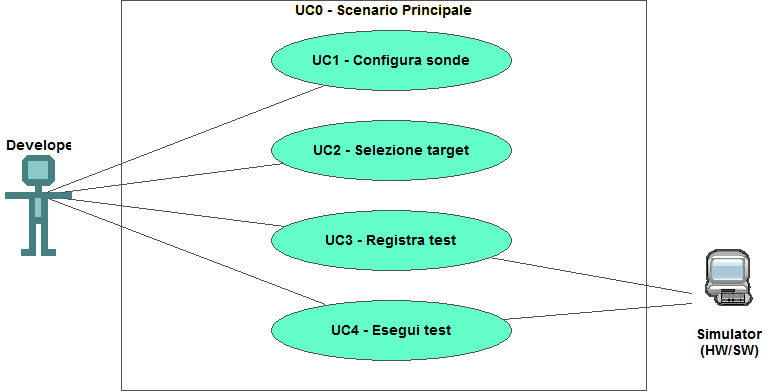
\includegraphics[width=0.9\columnwidth]{usecase/scenario-principale} 
    \caption{Use Case - UC4: invio e-mail}
\end{figure}


\begin{usecase}{4}{Automazione dell'invio di e-mail} 
    \usecaseactors{Programmatore, Sistema di posta elettronica} 
    \usecasepre{I siti web contenuti nel database hanno ricevuto una valutazione} 
    \usecasedesc{Il sistema invia automaticamente e-mail personalizzate ai proprietari dei siti con punteggi di qualità bassi, offrendo servizi di miglioramento} 
    \usecasepost{Le e-mail vengono inviate con successo ai destinatari} 
    \label{uc:invio-e-mail} 
\end{usecase}

\section{Tracciamento dei requisiti}

Da un'attenta analisi dei requisiti e degli use case effettuata sul progetto è stata stilata la tabella che traccia i requisiti in rapporto agli use case.\\
Sono stati individuati diversi tipi di requisiti e si è quindi fatto utilizzo di un codice identificativo per distinguerli.\\
Il codice dei requisiti è così strutturato R(F/Q/V)(N/D/O) dove:
\begin{enumerate}
	\item[R =] requisito
    \item[F =] funzionale
    \item[Q =] qualitativo
    \item[V =] di vincolo
    \item[N =] obbligatorio (necessario)
    \item[D =] desiderabile
    \item[Z =] opzionale
\end{enumerate}
Nelle tabelle \ref{tab:requisiti-funzionali}, \ref{tab:requisiti-qualitativi} e \ref{tab:requisiti-vincolo} sono riassunti i requisiti e il loro tracciamento con gli use case delineati in fase di analisi.

\newpage

\begin{table}%
\caption{Tabella del tracciamento dei requisti funzionali}
\label{tab:requisiti-funzionali}
\begin{tabularx}{\textwidth}{lXl}
\hline\hline
\textbf{Requisito} & \textbf{Descrizione} & \textbf{Use Case}\\
\hline
RFN-1     & L'interfaccia permette di configurare il tipo di sonde del test & UC1 \\
\hline
\end{tabularx}
\end{table}%

\begin{table}%
\caption{Tabella del tracciamento dei requisiti qualitativi}
\label{tab:requisiti-qualitativi}
\begin{tabularx}{\textwidth}{lXl}
\hline\hline
\textbf{Requisito} & \textbf{Descrizione} & \textbf{Use Case}\\
\hline
RQD-1    & Le prestazioni del simulatore hardware deve garantire la giusta esecuzione dei test e non la generazione di falsi negativi & - \\
\hline
\end{tabularx}
\end{table}%

\begin{table}%
\caption{Tabella del tracciamento dei requisiti di vincolo}
\label{tab:requisiti-vincolo}
\begin{tabularx}{\textwidth}{lXl}
\hline\hline
\textbf{Requisito} & \textbf{Descrizione} & \textbf{Use Case}\\
\hline
RVO-1    & La libreria per l'esecuzione dei test automatici deve essere riutilizzabile & - \\
\hline
\end{tabularx}
\end{table}%
